Après l'analyse de l'existant, nous avons décidé de développer le logiciel entièrement sans réutiliser un logiciel pré-existant. En effet, la reprise d'un code réalisé par une autre personne est aussi longue que de le développer soi-même. De plus, le logiciel doit répondre à de nombreux critères tel que la maintenabilité du code mais également avoir une architecture optimale, qui n'auraient pas forcément été présents dans le code repris. Cependant, nous nous sommes inspirés des différents articles portant sur des heuristiques pour l'IA.

\section{Architecture du projet}

La création d'un jeu comme Othello est considérable, pour faciliter le développement nous avons décidé de segmenter en briques fonctionnelles le projet. Le principe de la segmentation (voir figure \ref{glob}) en module est qu’ils sont tous indépendants et testables séparément. Nous comptons six segments : le logiciel, l'intelligence artificielle, le gestionnaire de fichiers, l'éditeur de plateau, le BenchMark et le gestionnaire de temps.

Les blocs IA et logiciel sont les plus importants et conséquents. Le second intérêt de cette architecture est que chaque module peut être remplacé par un autre plus ou moins équivalent sans compromettre l’intégrité et le bon fonctionnement du logiciel. Par exemple, pour le bloc de l’IA, si une personne de la communauté souhaite l’améliorer, il peut tout simplement coder le module IA et l’intégrer au logiciel pour le tester.

Nous avons également ajouté un module supplémentaire pour nous faciliter le développement et la compréhension d'erreurs pour un utilisateur "scientifique". Le module "ErrorLog" permet d'écrire dans le même fichier ("log.txt") les différentes erreurs rencontrées pendant l'utilisation actuelle du logiciel.

Développant en JAVA, les différents modules sont liés par le biais d’interfaces. Ainsi, chaque brique présentera une interface définie et dûment commentée qui représentera le comportement du module (sauf pour le BenchMark et ErrorLog qui ne possèdent qu'une à deux méthodes).


\begin{figure}[H]
\centering
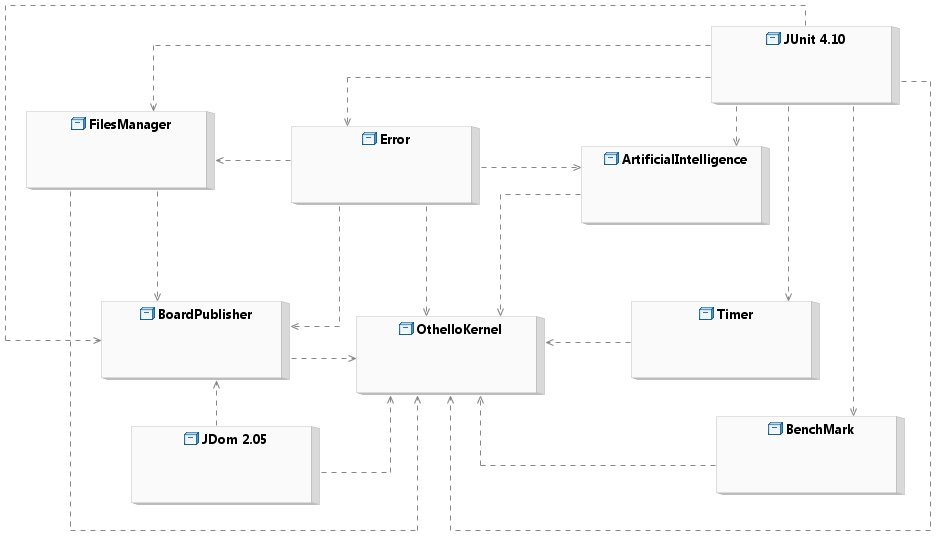
\includegraphics[scale=0.64]{Architecture/DiagrammeDependances.png}
\caption{Diagramme de dépendances}
\label{glob}
\end{figure}

\subsection{Logiciel}

C'est le module principal qui va gérer le fonctionnement complet du jeu. Il va intégrer tous les autres modules et lancer l'interface graphique permettant à l'utilisateur de jouer. Il gère l'accès et l'utilisation de ces derniers lors du déroulement du jeu.

Le logiciel (voir figures \ref{OthKer}) est lui-même composé de trois modules principaux : l'interface, les données et le contrôleur.
Ce dernier gère l'intégralité du projet. Il exploite tous les modules au bon moment pour chaque fonctionnalité le néccessitant.

De plus, il était prévu à la base de faire une vue en mode "shell" (sur le terminal) en plus de la vue graphique. Ainsi, nous avons géré l'intégralité du comportement général du jeu dans une classe abstraite. Pour chaque affichage différent du jeu, il suffit de créer un contrôleur qui spécialise celui-ci. C'est le cas de notre interface graphique qui est gérée par la classe "GameControllerGraphical" implémentant la classe abstraite "GameController". Ainsi pour gérer un affichage type "Shell", il suffirait de créer un fichier "GameControllerShell", en suivant l'exemple de "GameControllerGraphical", qui afficherait le jeu dans le terminal.

\subsection{Intelligences Artificielles}

Ce module (voir figure \ref{ia}) est la partie la plus compliquée et la plus importante à réaliser dans notre projet. En effet, il se compose de différentes IA qui ont des algorithmes distincts, chacune avec sa propre stratégie correspondant à un niveau de difficulté.


\begin{figure}[H]
\centering
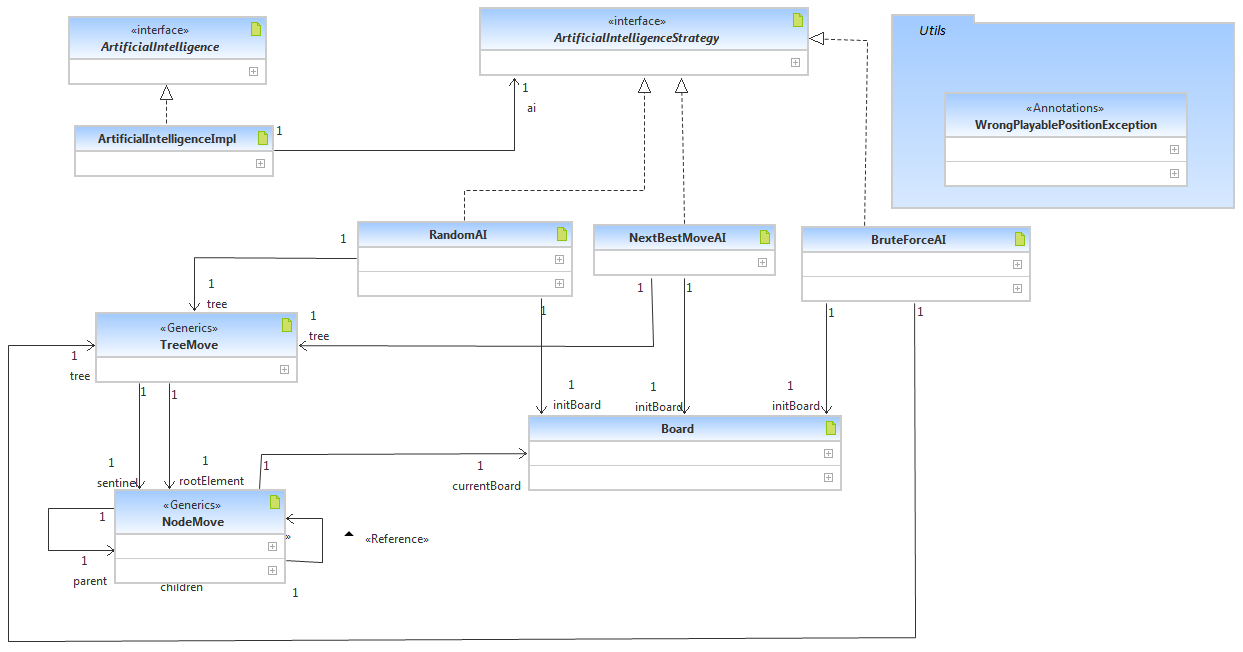
\includegraphics[scale=0.48]{Architecture/ArtificialIntelligenceLight.png}
\caption{Diagramme UML de classe du module d'intelligence artifcielle}
\label{ia}
\end{figure}

Pour les différents calculs des algorithmes, un pattern state avait été mis en place afin de représenter le plateau. Cependant, ce pattern rend les structures lourdes à allouer et à désallouer par la JVM ce qui va entraîner des surcharges de piles, des erreurs de désallocation du Garbage Collector de la JVM, ... Nous avons donc décidé de rendre la structure plus simple mais tout aussi efficace en utilisant simplement une énumération de pion pour représenter une case.

De plus, nous avons créé deux classes nous permettant de manipuler des arbres génériques. La généricité de ces arbres permet la réutilisation de ces classes par d'autres développeurs.

\subsection{Gestionnaire de Fichier}

Il permet de gérer et surtout de sécuriser les actions de lecture et d'écriture pour les différents accès aux fichiers. Il est essentiellement utilisé pour les actions de sauvegarde et de chargement des parties.



\begin{figure}[H]
\centering
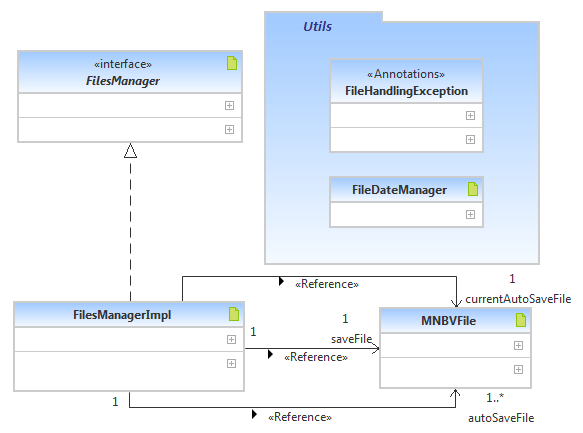
\includegraphics[scale=1.0]{Architecture/FilesManagerLight.png}
\caption{Diagramme UML de classe du module de gestion de fichier}
\label{gest}
\end{figure}


\subsection{Editeur de Plateau}

Ce module permet à l'utilisateur de générer un plateau qu'il pourra ensuite charger dans le logiciel pour jouer. Le plateau est personnalisable : la taille de la grille, la position et le nombre de pions de départ. Cette fonctionnalité est lancée dans la console système à partir du menu du jeu.

L'éditeur possède une partie correspondant à un modèle à savoir les classes Board et Player. Ces classes servent à récupérer les données utilisateur. Celles-ci sont ensuite utilisées par les classes LoadBoardFile et GenerateXML. La classe LoadBoardFile permet de récupérer une grille préconfigurée (fichier.grd). GenerateXML permet grâce à la bibliothèque JDOM 2.05 (\url{http://www.jdom.org/}) de générer un document xml bien formaté. Ce document correspond à notre fichier de sauvegarde.

\begin{figure}[H]
\centering
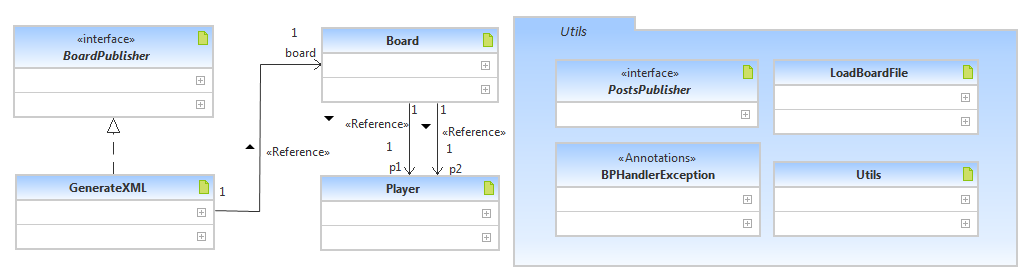
\includegraphics[scale=0.58]{Architecture/BoardPublisherLight.png}
\caption{Diagramme de classe du module éditeur de plateau}
\label{edit}
\end{figure}

\subsection{BenchMark}

Cette brique permet de lancer une série d'algorithmes compliqués et gourmands en ressources qui prendra un temps plus ou moins long selon la machine. A partir de ce temps, on peut connaître la puissance de l'ordinateur qui exécute le programme. Par manque de temps, nous n'avons pas pu implémenter l'utilisation de ce module dans le logiciel. Cela nous aurait permis de modifier l'utilisation de certains algorithmes de l'IA en fonction des capacités disponibles.

Ce module est basé sur un travail réalisé par les scientifiques Roldan Pozo et Bruce Miller : SciMark 2.0. Ce logiciel, libre de droit, réalise plusieurs calculs et établit un score selon les résultats. Par manque de temps, nous n'avons pas pu nous pencher d'avantage sur les calculs utilisés.

Ainsi, notre brique reprend ce module et permet de faire une liaison entre celui-ci et le logiciel qui va l'utiliser. Pour cela, nous utilisons une interface qui va informer le logiciel de l'état d'avancement du BenchMark, celui-ci durant environ 30 secondes.

\begin{figure}[H]
\centering
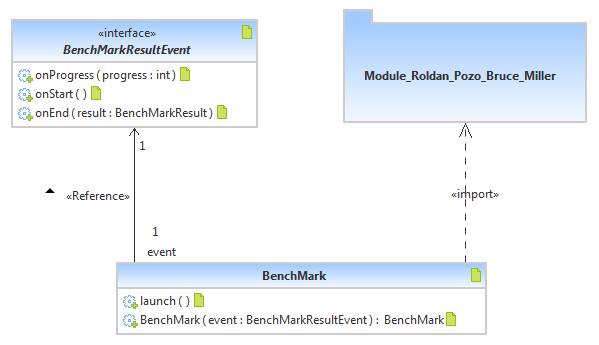
\includegraphics[scale=1]{Architecture/BenchMark.png}
\caption{Diagramme UML de classe du module de BenchMark}
\label{bench}
\end{figure}

\subsection{Gestionnaire de Temps}

Cette partie \ref{time} propose les fonctionnalités de chronomètre et de minuteur. Celles-ci sont utilisées pour limiter le temps de calcul de l'IA et minuter le jeu.

Le minuteur déclenche une action dès que le temps passé en paramètre de la méthode est écoulé. Cet évènement est récupéré par le logiciel qui peut ensuite réaliser le traitement associé.

Le chronomètre fonctionne à partir de l'horloge système, plus particulièrement sur le temps écoulé en millisecondes. Après déclenchement et jusqu'à sa réinitialisation, le gestionnaire renvoie la différence du temps écoulé par rapport au temps du lancement.

\begin{figure}[H]
\centering
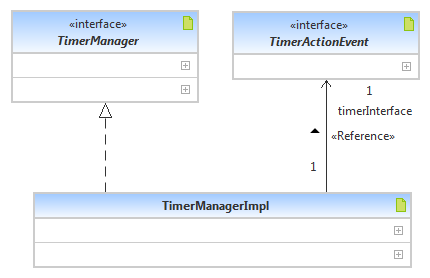
\includegraphics[scale=0.85]{Architecture/PdpTimerLight.png}
\caption{Diagramme de classe du module de gestion de temps}
\label{time}
\end{figure}
